\documentclass{scrartcl}
\usepackage{amsmath,amsfonts,amsthm,bm,graphicx}
\usepackage{tikz,pgfplots}
\usepackage{listings}
\usepackage{stmaryrd}
\usepackage{xcolor}
\usepackage{fdsymbol}
\usepackage{rotating}
\usepackage{listings}
\usepackage{hyperref}

\pgfplotsset{width=15cm,compat=1.18}
\allowdisplaybreaks
\setlength{\parindent}{0pt}

\title{Exercize 1: Matlab Basics}
\subtitle{Angewandte Modellierung 25}
\author{Carl Colmant}
\date{\today}
\begin{document}
\maketitle
\section*{Differential Equation}

\subsection*{a)}
Gegeben ist eine Differentialgleichung:
\begin{equation*}
    x''+\omega^2x=0 , \omega>0
\end{equation*}
mit den Randbedingungen:
\begin{equation*}
    x(0)=0,\quad x'(0)=1
\end{equation*}
Eine Möglichkeit ist die Verwendung von \texttt{dsolve} in Matlab. Womit Differentialgleichungen mit gegebenen Bedingungen gelöst werden können.\\
Somit kann die Differentialgleichung in Matlab wie folgt gelöst werden:
\begin{lstlisting}[language=Matlab, caption=Symbolic Math]
    %Symbolic Math:
    syms x(t) omega positive % Symbole

    eq = diff(x, t, 2) + omega^2 * x == 0; % Equation

    Dx = diff(x, t); % first differential
    % Conditions for the Equation
    cond = [x(0) == 0, Dx(0) == 1]; 

    sol = dsolve(eq, cond);
\end{lstlisting}

Eine andere Möglichkeit ist die Verwendung von \texttt{ode45} in Matlab. Womit Differentialgleichungen mit gegebenen Bedingungen numerisch gelöst werden können.\\
Dazu muss man die symbolische Funktion in eine numerische Funktion umwandeln und einen Werte Bereich für die x Achse definieren. Außerdem muss für $\omega$ ein wert eingesetzt werden \\
\begin{lstlisting}[language=Matlab, caption=Numeric Math]
    % numeric Math:
    % Parameter
    omega_val = 1;  % Setze z.B. omega = 2

    % System 1. Ordnung: x1 = x, x2 = dx/dt
    f = @(t, y) [y(2); -omega_val^2 * y(1)];

    % Anfangswerte: x(0) = 0, dx/dt(0) = 1
    y0 = [0; 1];

    % Zeitintervall
    tspan = [0, 5];

    % Numerische Lösung
    [t_num, y_num] = ode45(f, tspan, y0);
    \end{lstlisting}

\subsection*{b)}
Gegeben ist die Differentialgleichung:
\begin{equation*}
    x'=-\alpha x,  \alpha>0
\end{equation*}
mit den Randbedingungen:
\begin{equation*}
    x(0)=1
\end{equation*}

Die Lösung der Differentialgleichung ist fast identisch zu der Lösung der ersten Differentialgleichung. Lediglich die Funktion und die Bedingungen müssen angepasst werden.\\
Die Differentialgleichung kann in Matlab wie folgt gelöst werden:
\begin{lstlisting}[language=Matlab, caption=Symbolic Math]
    % Symbolic Math:

    syms x(t) a positive %Symbole
    
    eq = diff(x, t) == -a*x(t); % Die Differential Gleichung
    
    cond = x(0) == 1; %Die Bedinungen
    
    sol = dsolve(eq,cond); % Berechnung
\end{lstlisting}

Auch die Lösung mit \texttt{ode45} ist fast identisch. Meine Fassung ist etwas gekürzt.\\
\begin{lstlisting}[language=Matlab, caption=Numeric Math]
    %Numeric Math:
    a = 2; %für die numerische Berechnung muss alpha fest sein
    f = @(t,x) -a*x; % die funktion zur numerischen berechnung
    y0 = 1; % die bedingung

    [t_num, y_num] = ode45(f,[0,10], y0); %berechnung
\end{lstlisting}

\subsection*{Plotting}
Die Plots der beiden Differentialgliechung sind fast identisch und der Code wurde von Chatgpt generiert. Hier der Code für die zweite Differentialgleichung.\\
\begin{lstlisting}[language=Matlab, caption=Plot]
    %Plot von Chat GPT erstellt
    figure
    plot(t_num, y_num(:,1), 'b', 'LineWidth', 2)
    hold on
    fplot(subs(sol, a, 2), [0,10], 'r--', 'LineWidth', 2) %
    legend('Numerisch (ode45)', 'Symbolisch')
    xlabel('t')
    ylabel('x(t)')
    title('Vergleich: symbolisch vs. numerisch')
    grid on
\end{lstlisting}

Mithilfe dieses Codes erhält man die folgenden plots:\\
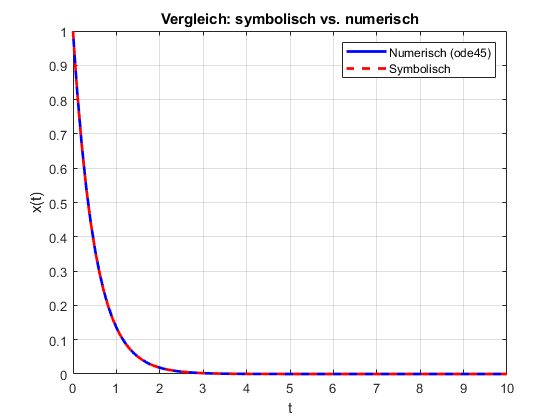
\includegraphics[scale=0.6]{radoactiv.png}\\
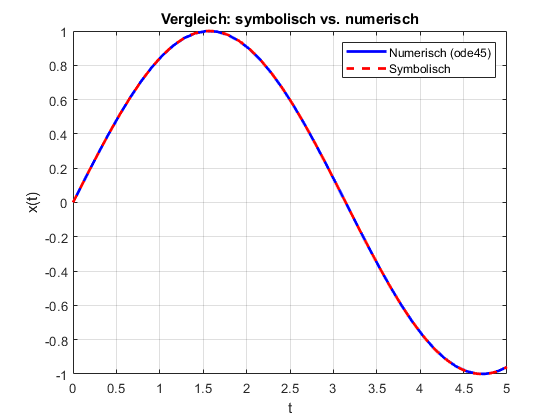
\includegraphics[scale=0.6]{pendel.png}\\

\section*{Simulink}
\subsection*{1.}
Für Die Sinus Simulation ist das ganze nicht sehr kompliziert. Man setzt in die Sinus Blocks die Parameter wie in der Aufgabe und verbindet alles so wie auf dem Bild. Das einzige Was noch zu tun ist ist die Schritt weite anzupassen damit die entstehende Kurve schön glat aussieht.\\ 
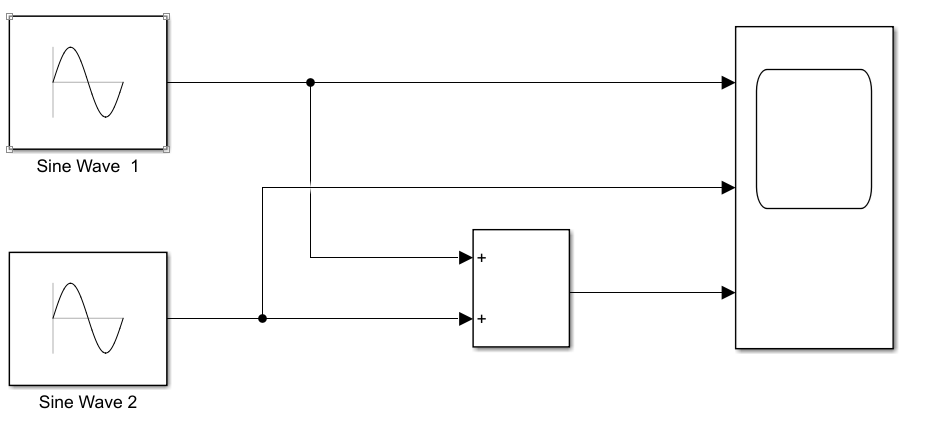
\includegraphics[scale=0.6]{Sinussim.png}
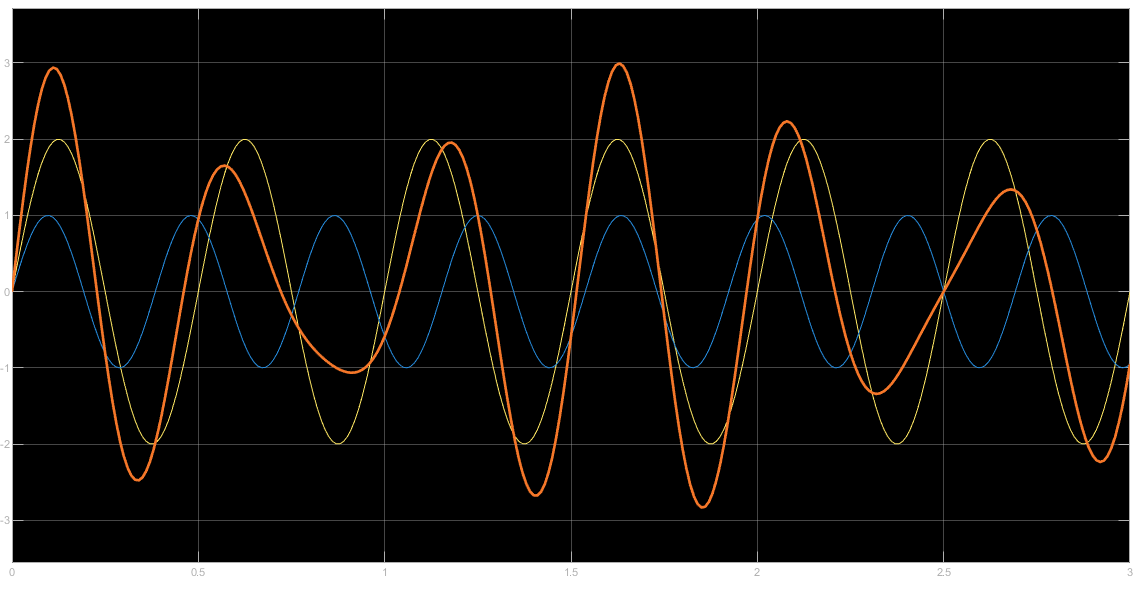
\includegraphics[scale=0.47]{Sinusplot.png}\\

\subsection*{2.}
Auch hier ist der Aufbau nicht besonders kompliziert. Man findet aber ein paar der Einstellungen nicht die auf dem Aufgabenblatt stehen und ich musste  einen 'Rate Transition' Block hinzufügen. Zur letzt so viele der Einstellungen in den Submenü des Spectrum Analyzers suchen und anpassen. Das führt dann zu folgenden Subsystemen:\\
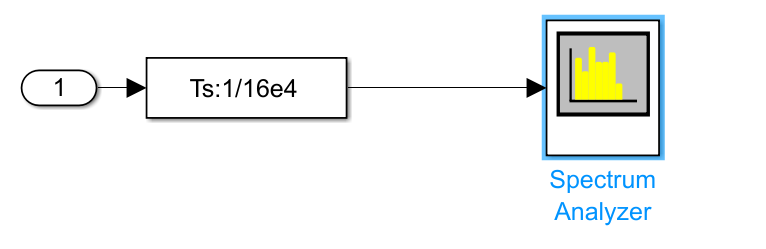
\includegraphics[scale=0.6]{Spectrum_Viewer.png}\\
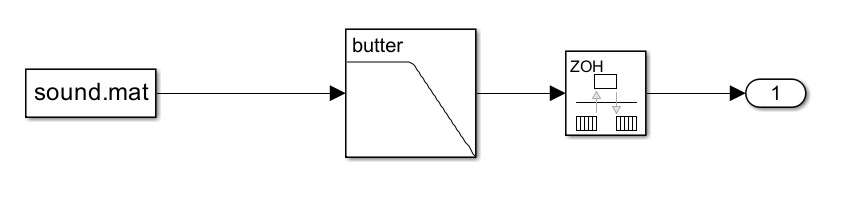
\includegraphics[scale=0.6]{Sound_Source.png} \\
und zu folgenden plots nach einer simulation:\\
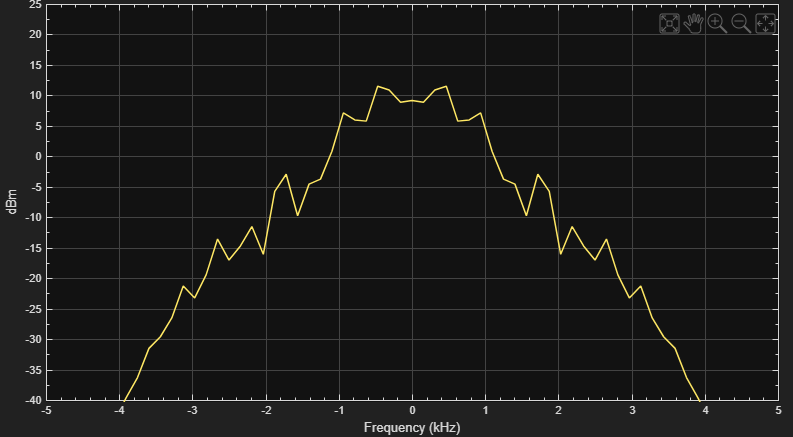
\includegraphics[scale=0.6]{Spectrumsim.png}\\

Falls noch Unklarheiten bestehen oder man sich denn Code noch mal angucken will, habe ich dafür ein Github Repository erstellt.\\
\url{https://github.com/7hands/Angewandte-Modellierung-25-Colmant}\\
Das Repository enthält alle Matlab und Simulink Dateien die ich für dieses Modul bearbeitet habe bzw benutzt habe. Das Repository ist natürlich öffentlich.

\end{document}